\section{Imitation Dynamics}
The second evolutionary dynamic to be presented is that of \textit{Imitation Dynamics}. In this case, the new distribution of the population is not calculated strictly as a function of the fitness of each strategy for each generation. Instead, a simpler and perhaps more realistic logic is adopted: in each generation, we identify the strategy (or, in case of a tie, the strategies) that performed best. Then, given a defined number \( K \) of players who change strategy per generation, \( K \) non-optimal strategy players are randomly selected and each adopts one of the optimal strategies, again randomly, in the case of ties.

It is important to highlight that the selection is only made among players who are not already using an optimal strategy, and not among all players in the population. We consider this to reflect reality more accurately --- if a player is already following an optimal strategy, why would they consider changing? This choice has some consequences on the results that are presented below.

To determine the optimal strategy, a score calculation similar to that used in the fitness dynamics case is employed, in order to save computational time. That is, matches between every player are not actually simulated; instead, scores are calculated based on the payoffs of each strategy against each other strategy and the corresponding population sizes.

As will be shown below during the theoretical presentation of the \texttt{TourTheImi} function, this process can be formulated using a Markov chain, where the states are the various possible population distributions, based on the sum of the initial populations (the total population) and the number of strategies involved in the process. The theoretical background is crucial to understand the following implementations: initially, we consider the \( r \)-state Markov chain, where each state represents the individual strategy of each player. For example, for \( N = 5 \) players and 3 strategies, a possible \( r \)-state is (11323). We then consider the \( s \)-states, where a state represents the population of each strategy; in the previous example, the \( s \)-state would be (212). Essentially, this involves grouping various \( r \)-states into one \( s \)-state, which, since we are not truly interested in each individual player but in the total population per strategy, is equivalent. It is shown that the process \( r(t) \) is lumpable and therefore that \( s(t) \) is a Markov chain. This theoretical knowledge is necessary for the implementation of \texttt{TourTheImi} below.

\subsection{The function TourSimImi}
The function that simulates the evolutionary tournament with imitation dynamics is implemented as
\[
[\text{POP}, \text{BST}] = \text{TourSimImi}(B, \text{Strategies}, \text{POP}_0, K, T, J, \text{mode}).
\]
The inputs and outputs of the function are similar to those of \texttt{TourSimFit}, with the additional argument \( K \), an integer value that specifies the number of players who change strategy per generation. The additional argument \texttt{mode} (the function runs with default value \texttt{"Individual"}) can take the values \texttt{"Individual"} and \texttt{"Total"}, and refers to the way in which the optimal strategy is selected: in the \texttt{"Individual"} case, the strategy of the best individual player is returned, while in the \texttt{"Total"} case, the strategy with the highest total score among the players using it is selected. The choice of mode yields significantly different results, as will be shown below.

\subsection{The function TourTheImi}
The \texttt{TourTheImi} function has the form
\[
P = \text{TourTheImi}(B, \text{Strategies}, \text{POP}_0, K, T, J, \text{mode})
\]
with arguments identical to the function \texttt{TourSimImi}, and output the transition matrix \( P \) of the Markov chain of the s-states. In reality, the initial population is used only to determine the total population size of the tournament (so it could simply be replaced by an argument \( N \)), and the number of generations \( J \) is not used at all.

For this analysis, we consider the s-states of the tournament as the number of players using each strategy. For example, for \( N = 9 \), we may have
\[
s_1 = \begin{bmatrix} 0 & 0 & 9 \end{bmatrix}, \quad s_2 = \begin{bmatrix} 0 & 1 & 8 \end{bmatrix},
\]
and so on. Depending on the \texttt{mode} argument, we expect the transition matrix to take different forms. For example, in \texttt{"Individual"} mode and with strategies \texttt{All\_D}, \texttt{All\_C}, and \texttt{TitForTat}, we expect the state
\[
\begin{bmatrix} 0 & 5 & 4 \end{bmatrix}
\]
to be absorbing, since there are no non-optimal players, and therefore it should have only one transition — to itself — with probability 1. In contrast, in the \texttt{"Total"} mode, this state would not be absorbing, as the \texttt{All\_C} strategy accumulates more total points.

Another function is also created:
\[
\text{AnalyzeMarkovChain}(P, \text{POP}_0, \text{Strategies}, \text{Title}),
\]
which is responsible for generating the state transition diagrams shown below. This function, based on the matrix \( P \) calculated by the \texttt{TourTheImi} function and the initial population \texttt{POP0}, classifies the states into transient, absorbing, and the initial state. It also further distinguishes between reachable and unreachable states based on the initial state. It generates a diagram of each state, where the state type is indicated with color, the population of each strategy is shown, the strategy names are labeled (as given by the \texttt{Strategies} argument), and the corresponding transition probabilities are displayed above each transition. The \texttt{Title} argument is the title of the resulting diagram.

\subsection{Simulations - Examples}
Παρακάτω παρουσιάζονται κάποιες προσομοιώσεις οι οποίες παράγονται από τις συναρτήσεις που περιγράφηκαν παραπάνω και παρουσιάζουν ενδιαφέρον. Η κάθε προσομοίωση βρίσκεται στο αρχείο example.m σε κατάλληλο Section και με Run Section προκύπτουν ακριβώς τα αποτελέσματα που παρουσιάζονται παρακάτω.
\subsubsection{1η Προσομοίωση - Παράδειγμα χρήσης των Tour\-The\-Imi, Analyze\-Markov\-Chain και Tour\-Sim\-Imi}
Στην πρώτη προσομοίωση \ref{fig:TourTheImi153} παρουσιάζεται η μαρκοβιανή αλυσίδα που προκύπτει για τις στρατηγικές $\begin{bmatrix}All\_D&All\_C&TitForTat\end{bmatrix}$ σε μείγμα $\begin{bmatrix}1&5&3\end{bmatrix}$.
Από το διάγραμμα που προκύπτει παρατηρούμε ότι οι πιθανές απορροφητικές καταστάσεις είναι η $\begin{bmatrix}9&0&0\end{bmatrix}$, δηλαδή η επικράτηση της στρατηγικής $All\_D$, η $\begin{bmatrix}0&0&9\end{bmatrix}$, δηλαδή η επικράτηση της στρατηγικής $TitForTat$ και η $\begin{bmatrix}0&1&8\end{bmatrix}$, δηλαδή η επικράτηση της $TitForTat$ αλλά με επιβίωση της $All\_C$. Από τις πιθανότητες μετάβασης, που απεικονίζονται στα βέλη των μεταβάσεων, παρατηρούμε ότι η τελευταία απορροφητική κατάσταση έχει σημαντικά χαμηλότερη πιθανότητα να συμβεί σε σχέση με τις άλλες δύο. Ακόμη παρατηρούμε ότι οι καταστάσεις στις οποίες υπάρχουν μόνο οι συμπαθείς στρατηγικές ($All\_C$ και $TitForTat$), δηλαδή στρατηγικές οι οποίες ποτέ δεν λιποτακτούν πρώτες και άρα οι παίκτες των οποίων αποκτούν ίσα σκορ παίζοντας μεταξύ τους, μεταβαίνουν μόνο στον εαυτό τους καθώς δεν υπάρχουν παίκτες με σκορ χαμηλότερο του μεγίστου.

	\begin{figure}[h]
	      \centering
	      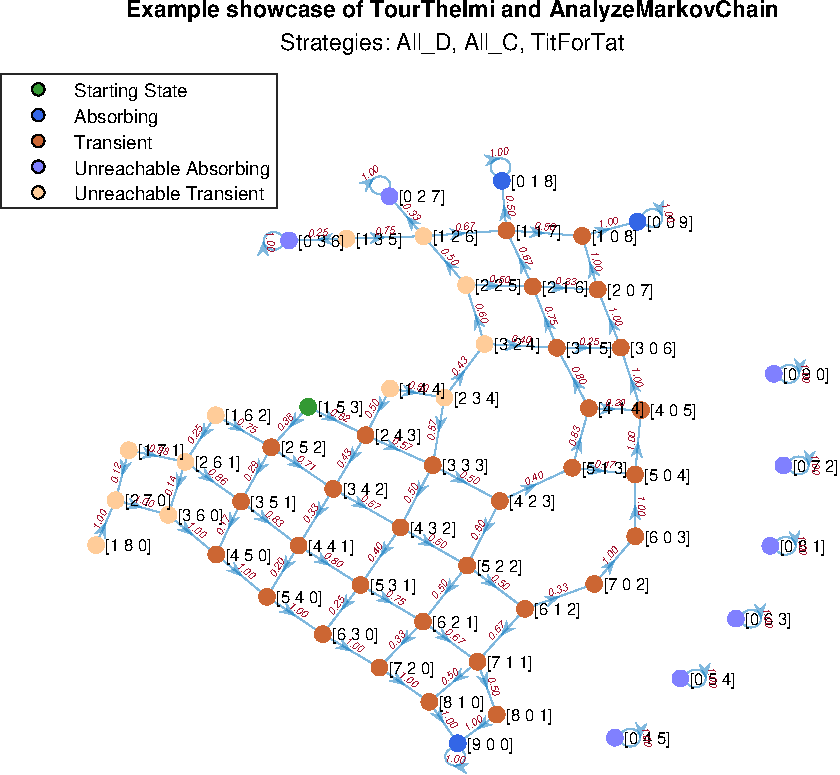
\includegraphics[width=0.95\textwidth]{Example showcase of TourTheImi and AnalyzeMarkovChain.pdf}
	      \caption{Example showcase of TourTheImi and AnalyzeMarkovChain}
	      \label{fig:TourTheImi153}
	\end{figure}
	
Στο Σχήμα \ref{fig:TourSimImi153} απεικονίζονται δύο εκτελέσεις της TourSimImi για το μείγμα στρατηγικών της παραπάνω προσομοίωσης. Παρατηρούμε ότι λόγω του τυχαίου τρόπου επιλογής των imitators, δηλαδή των παικτών που δεν έχουν την καλύτερη στρατηγική και αλλάζουν σε κάποια από τις καλύτερες, το τελικό μείγμα στρατηγικών είναι διαφορετικό για κάθε εκτέλεση του προγράμματος. Συγκεκριμένα στην (α) εκτέλεση παρατηρούμε $\begin{bmatrix}1&5&3\end{bmatrix} \rightarrow^* \begin{bmatrix}9&0&0\end{bmatrix}$ ενώ στην (β) εκτέλεση $\begin{bmatrix}1&5&3\end{bmatrix} \rightarrow^*	\begin{bmatrix}0&0&9\end{bmatrix}$, που όπως αναλύσαμε παραπάνω είναι πράγματι οι δύο πιο πιθανές απορροφητικές καταστάσεις.
	\begin{figure}[h]
		\centering
		\begin{subfigure}{.5\textwidth}
			\centering
	      	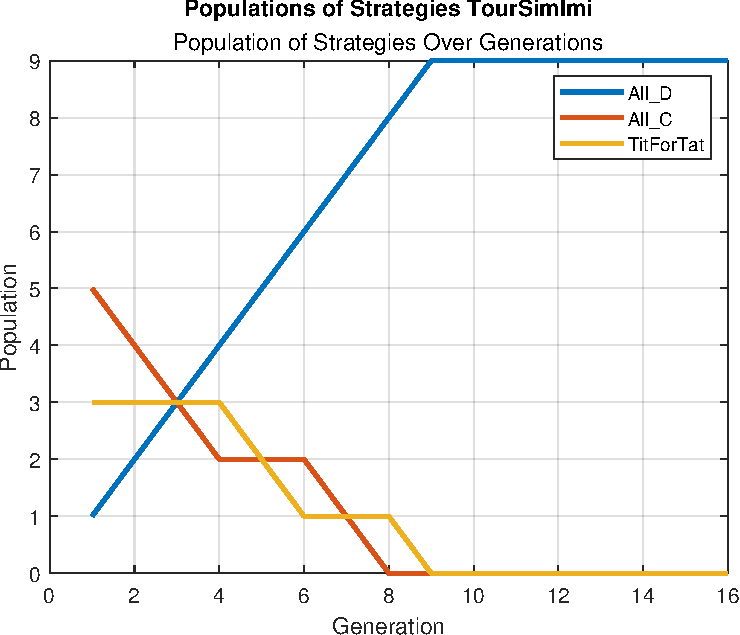
\includegraphics[width=.9\textwidth]{900.pdf}
			\caption{$\begin{bmatrix}9&0&0\end{bmatrix}$}
	      	\label{fig:900}
		\end{subfigure}%
		\begin{subfigure}{.5\textwidth}
			\centering
	      	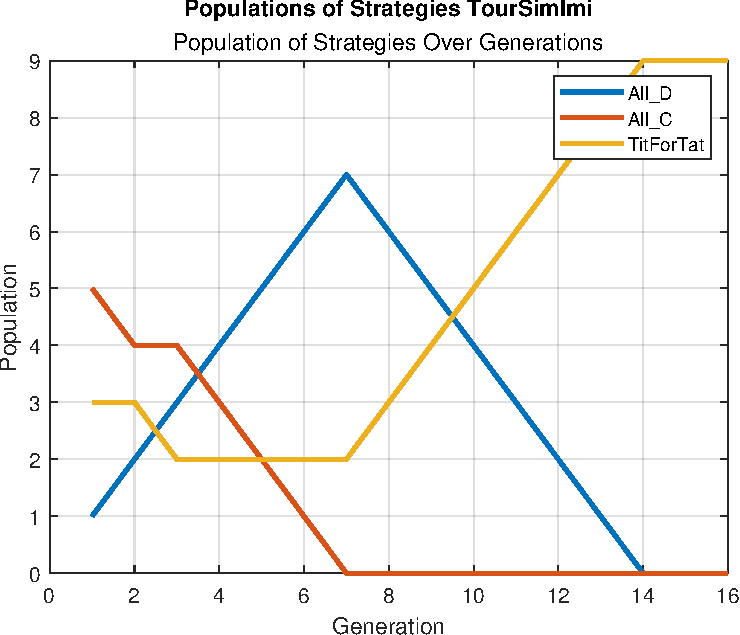
\includegraphics[width=0.90\textwidth]{009.pdf}
			\caption{$\begin{bmatrix}0&0&9\end{bmatrix}$}
	      	\label{fig:009}
		\end{subfigure}
		\caption{Absorbing States may differ even for the same Starting State}
		\label{fig:TourSimImi153}
	\end{figure}

\subsubsection{2η Προσομοίωση - Δοκιμή προεπιλεγμένης μεθόδου (Individual) για τον προσδιορισμό της καλύτερης στρατηγικής}
Στις δύο επόμενες προσομοιώσεις επιχειρείται να παρουσιαστεί η διαφορά στα αποτελέσματα που προκαλεί η διαφορετική μεθοδολογία επιλογής της καλύτερης στρατηγικής. Αρχικά (\ref{fig:TourTheImiIndividual}) παρουσιάζεται η μαρκοβιανή αλυσίδα που προκύπτει για αρχικό μείγμα στρατηγικών $\begin{bmatrix}1&4&5\end{bmatrix}$ και επιλογή μεθόδου ``Individual'', δηλαδή επιλογή της καλύτερης στατηγικής με σύγκριση των payoffs των στρατηγικών με παιχνίδια ένας εναντίον ενός για κάθε ζεύγος στρατηγικών.

Το αποτέλεσμα είναι αντίστοιχο αυτού της πρώτης προσομοίωσης \ref{fig:TourTheImi153}. Με λίγη παρατήρηση μπορούμε να οραματιστούμε μία νοητή καμπύλη μεταξύ των κορυφών των καταστάσεων $\begin{bmatrix}8&0&2\end{bmatrix}, \begin{bmatrix}6&1&3\end{bmatrix}, \begin{bmatrix}4&2&4\end{bmatrix}, \begin{bmatrix}2&3&5\end{bmatrix}$ η οποία χωρίζει τις λεκάνες απορροής των συμπαθών και των μη-συμπαθών στρατηγικών. Αν βρεθούμε σε κατάσταση κάτω από αυτή την καμπύλη θα καταλήξουμε στην απορροφητική κατάσταση επικράτησης της ``All\_D'', ενώ από κατάσταση πάνω από αυτή την καμπύλη θα καταλήξουμε σε μία από τις απορροφητικές καταστάσεις των συμπαθών στρατηγικών.
	\begin{figure}[h]
	      \centering
	      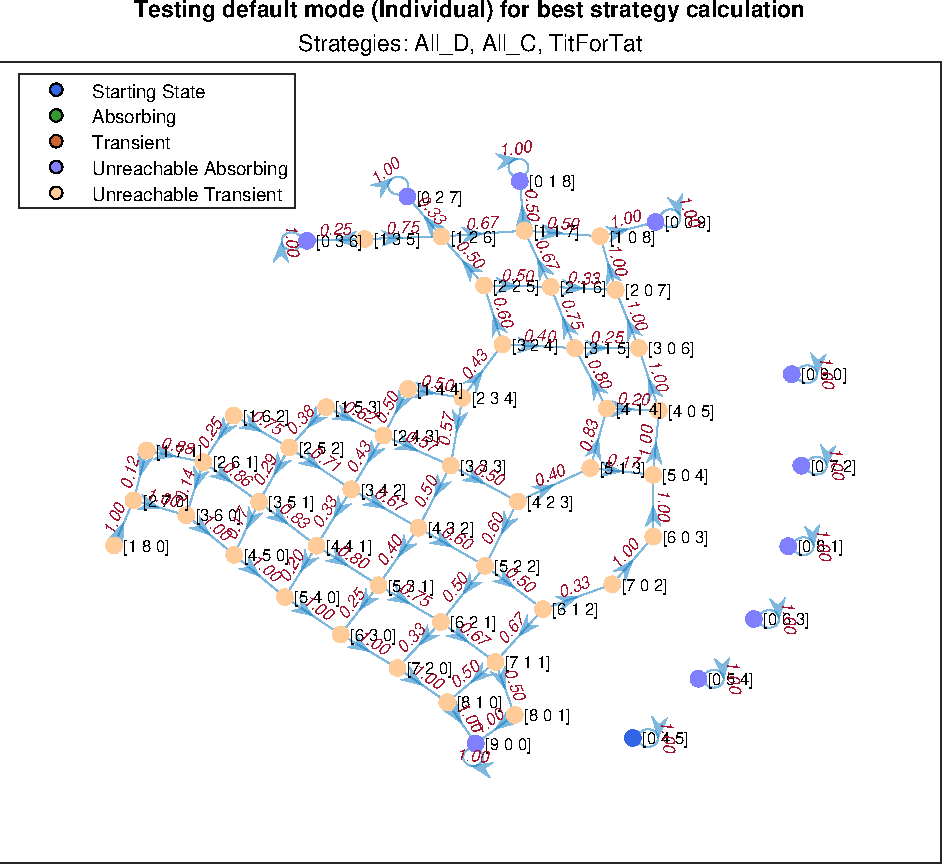
\includegraphics[width=0.95\textwidth]{Testing default mode (Individual) for best strategy calculation.pdf}
	      \caption{Testing default mode (``Individual'') for best strategy calculation with $POP0=\begin{bmatrix}1&4&5\end{bmatrix}$}
	      \label{fig:TourTheImiIndividual}
	\end{figure}
\subsubsection{3η Προσομοίωση - Δοκιμή μεθόδου ``Total'' για τον προσδιορισμό της καλύτερης στρατηγικής}
Στην τρίτη προσομοίωση (\ref{fig:TourTheImiTotal}) για ίδιο αρχικό μείγμα στρατηγικών $\begin{bmatrix}1&4&5\end{bmatrix}$ και επιλογή μεθόδου ``Total'', δηλαδή σύγκριση των payoffs των παικτών που προκύπτουν σε κάθε state από Axelrod με τους πληθυσμούς του state και επιλογή ως καλύτερη στρατηγική της στρατηγικής του παίκτη με το μεγαλύτερο συνολικό payoff.

Σε αντίθεση με την προηγούμενη προσομοίωση (\ref{fig:TourTheImiIndividual}) εδώ παρατηρούμε ότι το διάγραμμα είναι χωρισμένο σε τρεις ξεχωριστούς υπογράφους.
Ο πρώτος υπογράφος, αυτός που περιλαμβάνει την αρχική κατάσταση, είναι ο μόνος που περιλαμβάνει προσεγγίσιμη απορροφητική κατάσταση (την $\begin{bmatrix}0&0&10\end{bmatrix}$), η οποία είναι η επικράτηση της ``TitForTat''. Αυτό συμβαίνει διότι κατά την εύρεση της καλυτερης στρατηγικής στο mode ``Total'' οι συμπαθείς στρατηγικές συνεργάζονται μεταξύ τους και υπερνικούν λόγω του μεγαλύτερου πλήθους τους το προβάδισμα που δίνει η λιποταξία στην ``All\_D''
Ο δεύτερος υπογράφος είναι αυτός που περιλαμβάνει την απορροφητική κατάσταση που επικρατεί η ``All\_D'' ($\begin{bmatrix}10&0&0\end{bmatrix}$), η οποία όμως είναι μη προσπελάσιμη όπως και οι μεταβατικές καταστάσεις όλου του υπογράφου, για τον λόγο που περιγράφηκε παραπάνω.
Τέλος ο τρίτος υπογράφος είναι αυτός που περιλαμβάνει την απορροφητική κατάσταση που επικρατεί η ``All\_C'' ($\begin{bmatrix}0&10&0\end{bmatrix}$), η οποία είναι επίσης μη προσπελάσιμη όπως και οι μεταβατικές καταστάσεις όλου του υπογράφου, για τον λόγο που περιγράφηκε παραπάνω.

	\begin{figure}[h]
	      \centering
	      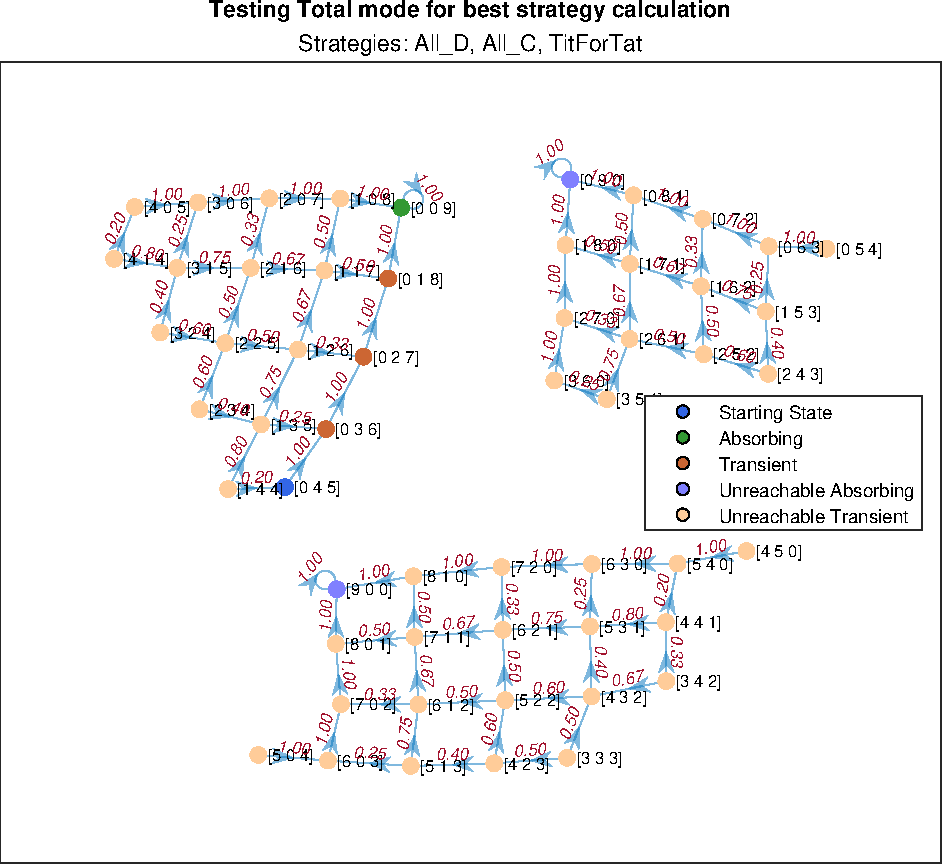
\includegraphics[width=0.95\textwidth]{Testing Total mode for best strategy calculation}
	      \caption{Testing ``Total'' mode for best strategy calculation with $POP0=\begin{bmatrix}1&4&5\end{bmatrix}$}
	      \label{fig:TourTheImiTotal}
	\end{figure}
